\documentclass[DM, lsstdraft, toc]{lsstdoc}
% lsstdoc documentation: https://lsst-texmf.lsst.io/lsstdoc.html
\usepackage{geometry}
\usepackage{longtable,booktabs,graphicx}
\usepackage{enumitem}
\usepackage{arydshln}

% Generated by Makefile
\input{meta}

% Package imports go here.

% Local commands go here.
\newcolumntype{R}[1]{>{\raggedleft\arraybackslash}p{#1}}
\newcolumntype{L}[1]{>{\raggedright\arraybackslash}p{#1}}

\providecommand{\tightlist}{
  \setlength{\itemsep}{0pt}\setlength{\parskip}{0pt}}

% If you want glossaries, uncomment:
% \input{aglossary.tex}
% \makeglossaries

\title{Characterization Metric Report: Science Pipelines Version 23.0.0}
% \setDocSubtitle{Optional subtitle}

\author{Jeff Carlin}

\setDocRef{DMTR-351}
\setDocUpstreamLocation{\url{https://github.com/lsst-dm/DMTR-351}}
\date{\vcsDate}
% \setDocCurator{The Curator of this Document}

\setDocAbstract{%
This brief report describes measurements of data quality metrics that were carried out for release v23.0.0 of the LSST Science Pipelines.
The report for the previous version can be found in \citedsp{DMTR-311}.
}

% Revision history.
% Order: oldest first.
% Fields: VERSION, DATE, DESCRIPTION, OWNER NAME.
% See LPM-51 for version number policy.
\setDocChangeRecord{%
  \addtohist{1}{2021-12-14}{Unreleased.}{Jeff Carlin}
}

\begin{document}

\maketitle

In this Report, we characterize the performance of the Rubin Observatory Science Pipelines Version 23.0.0. We illustrate the performance via metrics that are measured on the HSC-RC2 dataset. RC2 consists of 3 tracts of data taken from the HSC-SSP survey, and selected to provide a means of testing various ``pathological'' cases (e.g., difficult astrometric solutions, extremely good seeing that does not provide a well-sampled PSF, difficult fields for deblending, and large galaxies, among others). These three tracts each contain between 112--149 visits split between the HSC-G, HSC-R, HSC-I, HSC-Z, and HSC-Y (\emph{grizy}) filters. 

Version 23.0.0 represents the first data release production pipeline that relies entirely on Gen3 middleware; Gen2 middleware is now deprecated as of this release.

All metrics reported here were calculated using the \href{https://github.com/lsst/faro}{faro} metric calculation package, which is part of the standard pipeline builds. All of the underlying algorithms to calculate metrics within \texttt{faro} are the same as they were in v22.0.0 of the Science Pipelines, so most metrics should be expected to show similar results between v22 and v23 releases.

The metric calculation pipelines from \texttt{faro} were run on the RC2 tracts to derive the photometric, astrometric, and shape metrics that are reported here. We exclude the two astrometry metrics (AM3 and AF3) that concern residuals on 200-arcminute scales, since the individual tracts of RC2 do not span large enough spatial scales to enable these measurements. 

For comparison, we provide the \SRD required ``design'' value of each metric as defined in the Science Requirements Document \citedsp{LPM-17}.
%, and, where available, the target for this release as defined in the Data Management Development Milestone Roadmap \citedsp{LDM-240}. 
For context, the \SRD does not place any constraints on \emph{y}-band for these Key Performance Metrics (KPMs).  For the photometric metrics, there are only specifications for \emph{g}, \emph{r}, and \emph{i}. In the case of the ellipticity correlation metrics, there are specs only for \emph{r} and \emph{i}. The \emph{y}-band measurements are of interest primarily for historical tracking.

Some KPMs (e.g., PF1, AF1, AF2) involve thresholds that are different for ``design'', ``minimum'', and ``stretch'' specifications. Metrics in this report are all compared to the ``design'' thresholds. The assessment of these KPMs would be different if evaluated against different thresholds.

%The per-cycle target numbers come from the ``KPMs'' sheet of \href{http://ls.st/LDM-240}{LDM-240}.

\section{Note about sky backgrounds}\label{sec:notes}
In the v23.0.0 release of the Science Pipelines, the application of \texttt{skyCorr} (the global full focal plane background estimation) has been disabled for HSC data due to a bug in the pipelines that was being investigated at the time of the release (see \href{https://jira.lsstcorp.org/browse/DM-32827}{DM-32827} for details). This will be fixed before release v23.0.1. The absence of the \texttt{skyCorr} background corrections has a minor effect on coadd images, but all data products produced before the coaddition steps are unaffected. Of the metrics reported in this document, only the ellipticity correlations (Section~\ref{ellipticity-correlations}) TE1 and TE2 are measured on coadds.


\section{Metric monitoring dashboard}\label{sec:dashboard}

\begin{figure}[!t]
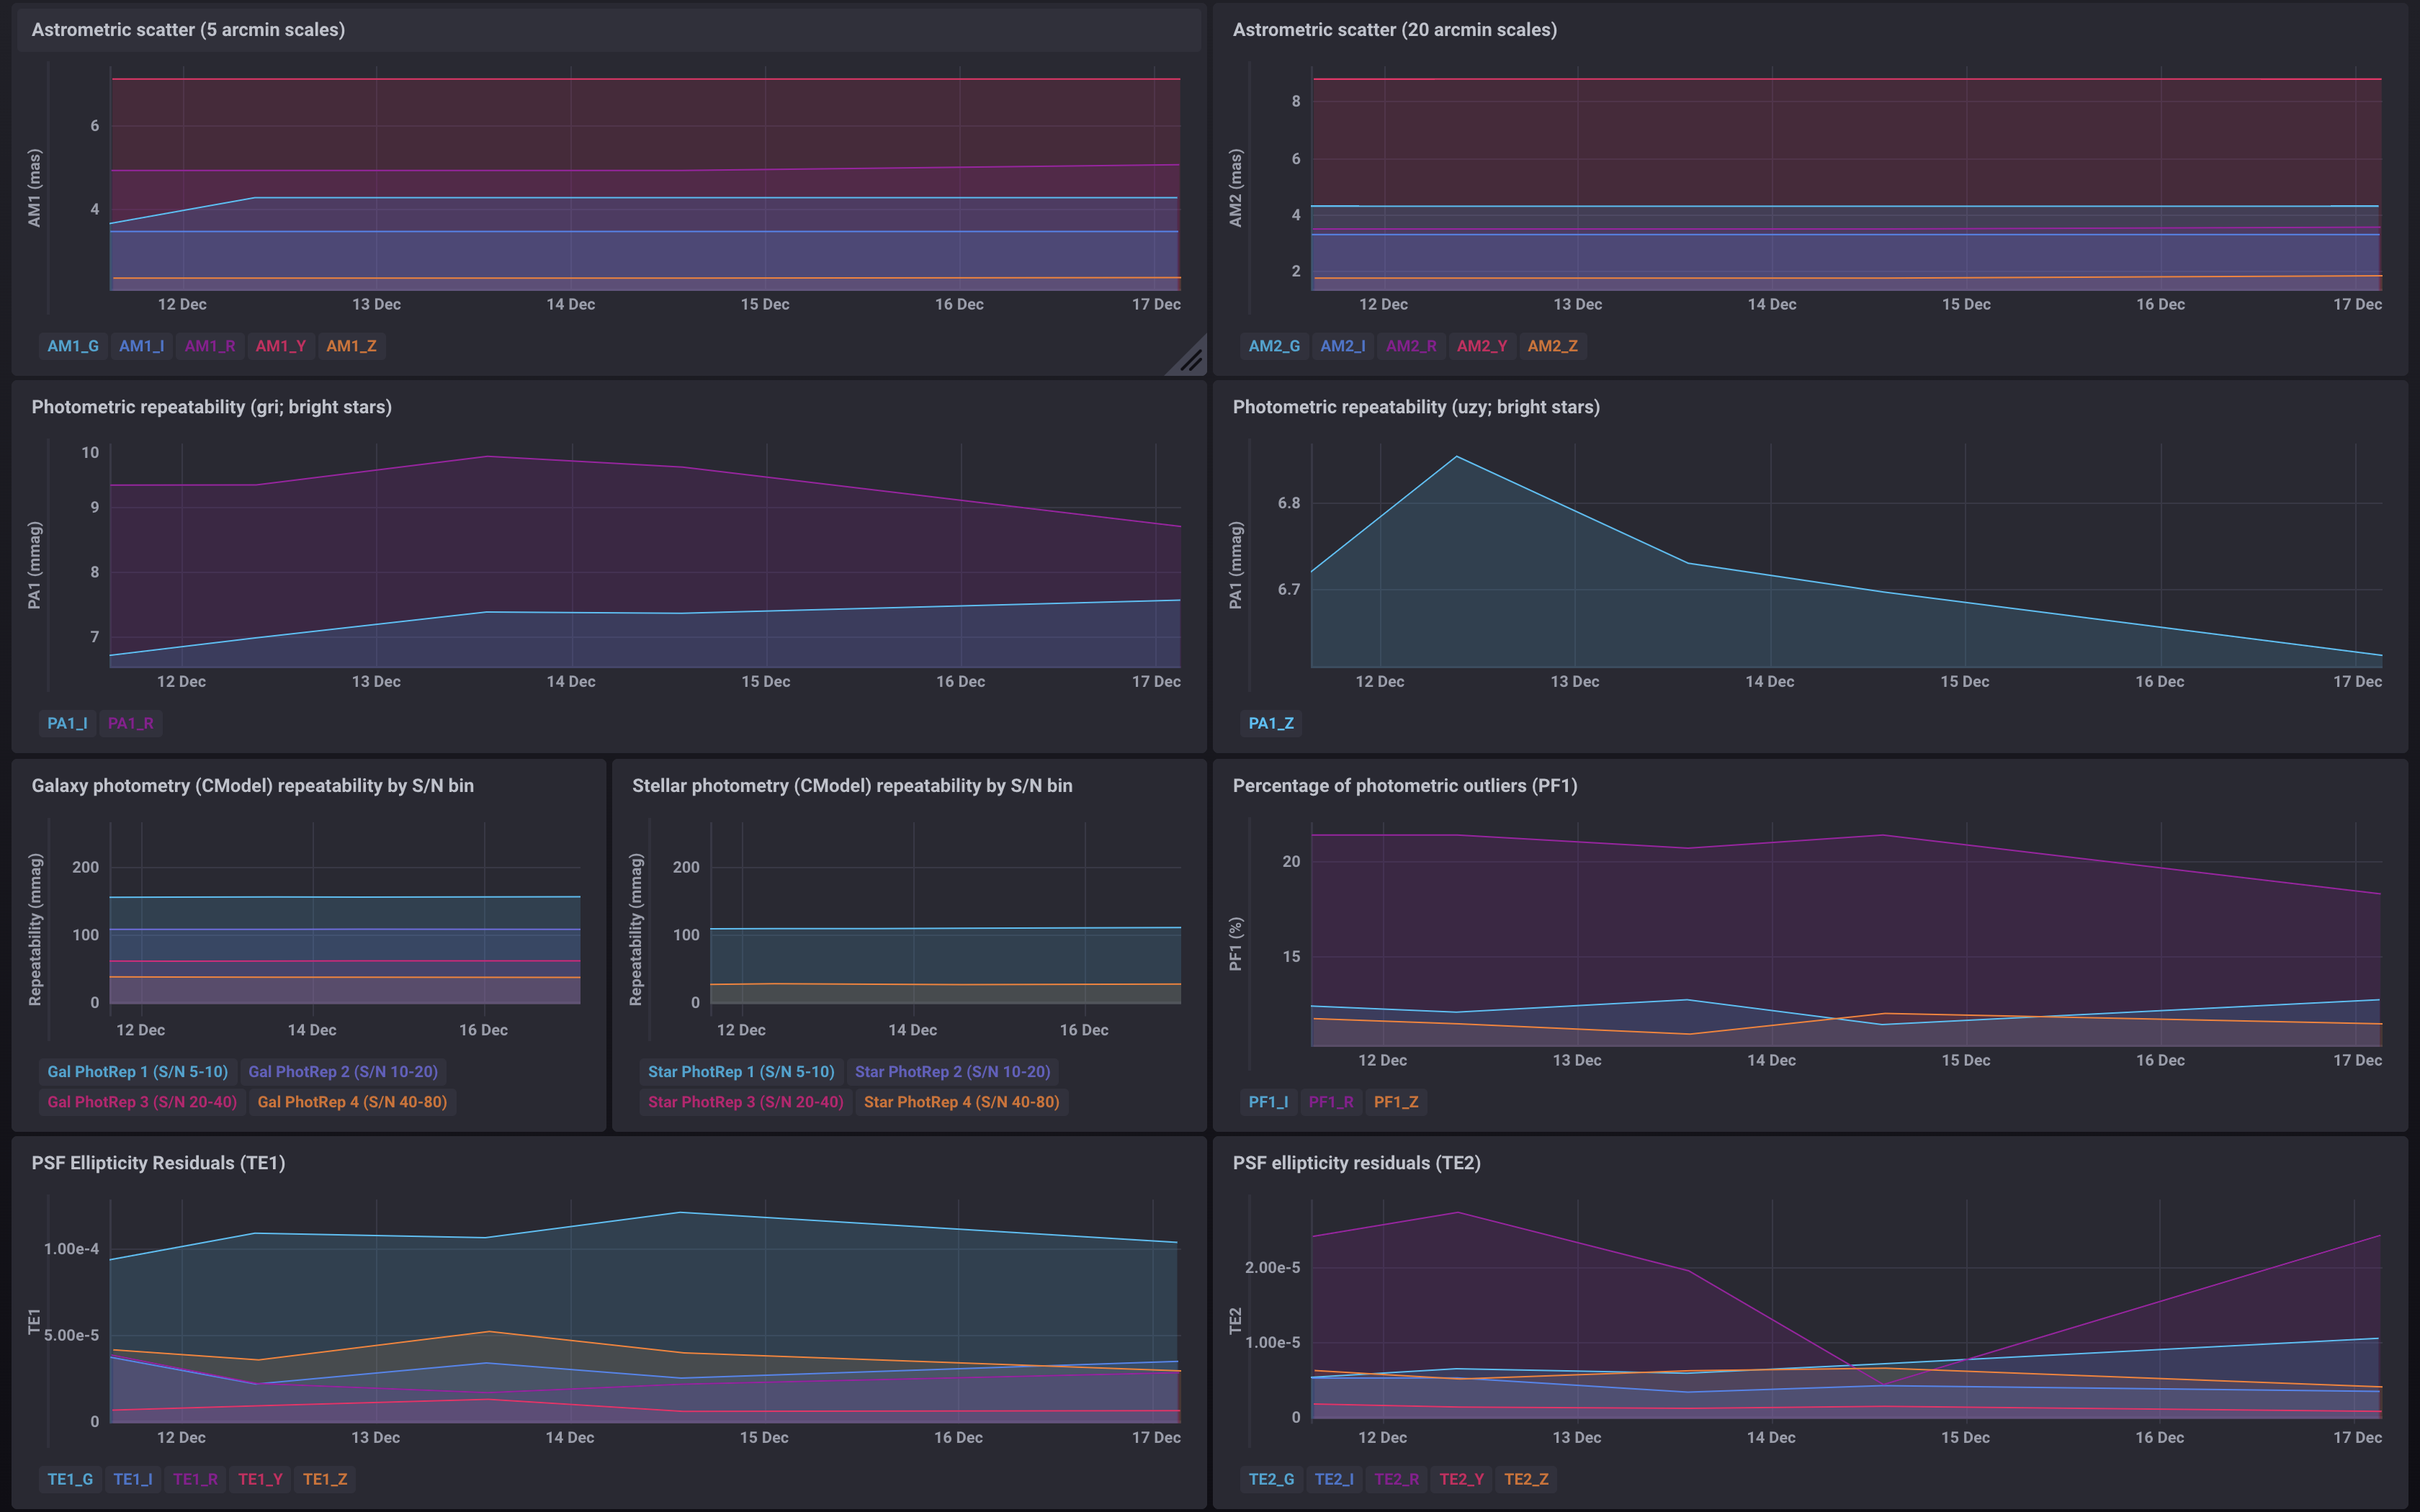
\includegraphics[width=1.0\columnwidth]{figures/verify_drp_metrics_dashboard_17dec2021.png}
\caption{A portion of the ``DRP metrics nightly CI Gen3 (rc2\_subset)'' dashboard on SQuaSH. This was recently created for daily tracking of metrics calculated on the \texttt{rc2\_subset} dataset via the nightly \texttt{verify\_drp\_metrics} CI job. The view shown here tracks metrics calculated each day for the past week. Although no changes in the science pipelines over the week displayed should contribute to changes in data quality, there are small fluctuations seen in many metrics. This is under investigation, but is likely due to small changes in data products brought about by non-deterministic behavior in some calibration algorithms.}
\end{figure}\label{fig:dashboard}

Since the previous Science Pipelines release, we have created a new dataset called \texttt{rc2\_subset}, which is a small selection of data from the RC2 dataset that includes only the 6 central detectors from 8 randomly chosen visits in each of the 5 filters \textit{grizy}. This dataset was created with the goal of covering a large enough area and including an ample number of sources for data quality monitoring in all five available HSC filters, but that is a small enough dataset that it can be reprocessed in its entirety in a nightly continuous integration (CI) job. This job has been dubbed \texttt{verify\_drp\_metrics}, and is automatically executed in Jenkins CI nightly. Data quality metrics calculated by \texttt{faro} are dispatched to SQuaSH (Science Quality System Harness; described in \citedsp{sqr-009}) and a dashboard displaying time-series plots of the metrics is updated daily to enable monitoring of data quality. Figure~\ref{fig:dashboard} shows a snapshot of the SQuaSH dashboard.


\section{Summary of performance metrics}

Because there have been no major changes in the data processing algorithms in the Science Pipelines between versions 22.0.0 and 23.0.0, the data quality metrics should be similar. Indeed, the astrometry metrics (Section~\ref{astrometric-performance}) are nearly identical between the previous (v22) and current (v23) Science Pipelines releases. The photometry metrics (Section~\ref{photometric-performance}) and ellipticity correlation metrics (Section~\ref{ellipticity-correlations}) show small differences between Release 22 and 23, most of which represent minor improvements in the metric values. A likely explanation for these minor improvements is the work done on ticket \href{https://jira.lsstcorp.org/browse/DM-31505}{DM-31505}, which updated the \texttt{FGCM} photometric calibration algorithms to better handle fields of view near the spatial edges of survey footprints. This likely affects RC2 data, because they consist of three distinct, isolated tracts, and thus have a relatively large fraction of ``edge'' data. It is obvious that improvements to the photometric \textit{calibration} will improve the measured photometry; the effects on ellipticity correlations likely arise due to the slightly different photometric calibrations altering the weights that are applied to individual frames during coaddition.


\section{Photometric Performance}\label{photometric-performance}

These photometric performance metrics are defined in LSS-REQ-0093 (\citeds{LSE-29}) and Table 14 of \citeds{LPM-17}. Values in this table represent the mean of the results reported by \texttt{faro} for the three tracts in RC2.

Any entries left blank are those for which we do not have data in the given filter for that dataset.

\begin{longtable}[]{@{}llllll@{}}
\toprule
\begin{minipage}[b]{0.12\columnwidth}\raggedright\strut
Metric\strut
\end{minipage} & \begin{minipage}[b]{0.06\columnwidth}\raggedright\strut
Unit\strut
\end{minipage} & \begin{minipage}[b]{0.14\columnwidth}\raggedright\strut
SRD Requirement -- Design\strut
\end{minipage} & \begin{minipage}[b]{0.12\columnwidth}\raggedright\strut
Release 22 Value (RC2) \strut
\end{minipage} & \begin{minipage}[b]{0.12\columnwidth}\raggedright\strut
Release 23 Value (RC2) \strut
\end{minipage} & \begin{minipage}[b]{0.17\columnwidth}\raggedright\strut
Comments\strut
\end{minipage}\tabularnewline
\midrule
\endhead
%\begin{minipage}[t]{0.12\columnwidth}\raggedright\strut
%procCalRep\strut
%\end{minipage} & \begin{minipage}[t]{0.06\columnwidth}\raggedright\strut
%mmag\strut
%\end{minipage} & \begin{minipage}[t]{0.14\columnwidth}\raggedright\strut
%\(\leq 3.0\)\strut
%\end{minipage} & \begin{minipage}[t]{0.14\columnwidth}\raggedright\strut
%3.5\strut
%\end{minipage} & \begin{minipage}[t]{0.12\columnwidth}\raggedright\strut
%---\strut
%\end{minipage} & \begin{minipage}[t]{0.12\columnwidth}\raggedright\strut
%---\strut
%\end{minipage} & \begin{minipage}[t]{0.17\columnwidth}\raggedright\strut
%Need simulations\strut
%\end{minipage}\tabularnewline
\begin{minipage}[t]{0.12\columnwidth}\raggedright\strut
PA1: \emph{u}\strut
\end{minipage} & \begin{minipage}[t]{0.06\columnwidth}\raggedright\strut
mmag\strut
\end{minipage} & \begin{minipage}[t]{0.14\columnwidth}\raggedright\strut
\(\leq 7.5\)\strut
\end{minipage} & \begin{minipage}[t]{0.12\columnwidth}\raggedright\strut
--- \strut
\end{minipage} & \begin{minipage}[t]{0.12\columnwidth}\raggedright\strut
--- \strut
\end{minipage} & \begin{minipage}[t]{0.17\columnwidth}\raggedright\strut
No data\strut
\end{minipage}\tabularnewline
\begin{minipage}[t]{0.12\columnwidth}\raggedright\strut
PA1: \emph{g}\strut
\end{minipage} & \begin{minipage}[t]{0.06\columnwidth}\raggedright\strut
mmag\strut
\end{minipage} & \begin{minipage}[t]{0.14\columnwidth}\raggedright\strut
\(\leq 5.0\)\strut
\end{minipage} & \begin{minipage}[t]{0.12\columnwidth}\raggedright\strut
7.6 \strut
\end{minipage} & \begin{minipage}[t]{0.12\columnwidth}\raggedright\strut
7.1 \strut
\end{minipage} & \begin{minipage}[t]{0.17\columnwidth}\raggedright\strut
\strut
\end{minipage}\tabularnewline
\begin{minipage}[t]{0.12\columnwidth}\raggedright\strut
PA1: \emph{r}\strut
\end{minipage} & \begin{minipage}[t]{0.06\columnwidth}\raggedright\strut
mmag\strut
\end{minipage} & \begin{minipage}[t]{0.14\columnwidth}\raggedright\strut
\(\leq 5.0\)\strut
\end{minipage} & \begin{minipage}[t]{0.12\columnwidth}\raggedright\strut
8.5\strut
\end{minipage} & \begin{minipage}[t]{0.12\columnwidth}\raggedright\strut
8.4\strut
\end{minipage} & \begin{minipage}[t]{0.17\columnwidth}\raggedright\strut
\strut
\end{minipage}\tabularnewline
\begin{minipage}[t]{0.12\columnwidth}\raggedright\strut
PA1: \emph{i}\strut
\end{minipage} & \begin{minipage}[t]{0.06\columnwidth}\raggedright\strut
mmag\strut
\end{minipage} & \begin{minipage}[t]{0.14\columnwidth}\raggedright\strut
\(\leq 5.0\)\strut
\end{minipage} & \begin{minipage}[t]{0.12\columnwidth}\raggedright\strut
9.2\strut
\end{minipage} & \begin{minipage}[t]{0.12\columnwidth}\raggedright\strut
8.7\strut
\end{minipage} & \begin{minipage}[t]{0.17\columnwidth}\raggedright\strut
\strut
\end{minipage}\tabularnewline
\begin{minipage}[t]{0.12\columnwidth}\raggedright\strut
PA1: \emph{z}\strut
\end{minipage} & \begin{minipage}[t]{0.06\columnwidth}\raggedright\strut
mmag\strut
\end{minipage} & \begin{minipage}[t]{0.14\columnwidth}\raggedright\strut
\(\leq 7.5\)\strut
\end{minipage} & \begin{minipage}[t]{0.12\columnwidth}\raggedright\strut
7.0\strut
\end{minipage} & \begin{minipage}[t]{0.12\columnwidth}\raggedright\strut
6.7\strut
\end{minipage} & \begin{minipage}[t]{0.17\columnwidth}\raggedright\strut
\strut
\end{minipage}\tabularnewline
\begin{minipage}[t]{0.12\columnwidth}\raggedright\strut
PA1: \emph{y}\strut
\end{minipage} & \begin{minipage}[t]{0.06\columnwidth}\raggedright\strut
mmag\strut
\end{minipage} & \begin{minipage}[t]{0.14\columnwidth}\raggedright\strut
\(\leq 7.5\)\strut
\end{minipage} & \begin{minipage}[t]{0.12\columnwidth}\raggedright\strut
8.0\strut
\end{minipage} & \begin{minipage}[t]{0.12\columnwidth}\raggedright\strut
7.9\strut
\end{minipage} & \begin{minipage}[t]{0.17\columnwidth}\raggedright\strut
\strut
\end{minipage}\tabularnewline
\begin{minipage}[t]{0.12\columnwidth}\raggedright\strut
PF1: \emph{u}\strut
\end{minipage} & \begin{minipage}[t]{0.06\columnwidth}\raggedright\strut
\%\strut
\end{minipage} & \begin{minipage}[t]{0.14\columnwidth}\raggedright\strut
\(\leq 20\)\strut
\end{minipage} & \begin{minipage}[t]{0.12\columnwidth}\raggedright\strut
---\strut
\end{minipage} & \begin{minipage}[t]{0.12\columnwidth}\raggedright\strut
---\strut
\end{minipage} & \begin{minipage}[t]{0.17\columnwidth}\raggedright\strut
No data\strut
\end{minipage}\tabularnewline
\begin{minipage}[t]{0.12\columnwidth}\raggedright\strut
PF1: \emph{g}\strut
\end{minipage} & \begin{minipage}[t]{0.06\columnwidth}\raggedright\strut
\%\strut
\end{minipage} & \begin{minipage}[t]{0.14\columnwidth}\raggedright\strut
\(\leq 20\)\strut
\end{minipage} & \begin{minipage}[t]{0.12\columnwidth}\raggedright\strut
12.0\strut
\end{minipage} & \begin{minipage}[t]{0.12\columnwidth}\raggedright\strut
10.7\strut
\end{minipage} & \begin{minipage}[t]{0.17\columnwidth}\raggedright\strut
\strut
\end{minipage}\tabularnewline
\begin{minipage}[t]{0.12\columnwidth}\raggedright\strut
PF1: \emph{r}\strut
\end{minipage} & \begin{minipage}[t]{0.06\columnwidth}\raggedright\strut
\%\strut
\end{minipage} & \begin{minipage}[t]{0.14\columnwidth}\raggedright\strut
\(\leq 10\)\strut
\end{minipage} & \begin{minipage}[t]{0.12\columnwidth}\raggedright\strut
14.5\strut
\end{minipage} & \begin{minipage}[t]{0.12\columnwidth}\raggedright\strut
14.0\strut
\end{minipage} & \begin{minipage}[t]{0.17\columnwidth}\raggedright\strut
\strut
\end{minipage}\tabularnewline
\begin{minipage}[t]{0.12\columnwidth}\raggedright\strut
PF1: \emph{i}\strut
\end{minipage} & \begin{minipage}[t]{0.06\columnwidth}\raggedright\strut
\%\strut
\end{minipage} & \begin{minipage}[t]{0.14\columnwidth}\raggedright\strut
\(\leq 10\)\strut
\end{minipage} & \begin{minipage}[t]{0.12\columnwidth}\raggedright\strut
16.0\strut
\end{minipage} & \begin{minipage}[t]{0.12\columnwidth}\raggedright\strut
14.5\strut
\end{minipage} & \begin{minipage}[t]{0.17\columnwidth}\raggedright\strut
\strut
\end{minipage}\tabularnewline
\begin{minipage}[t]{0.12\columnwidth}\raggedright\strut
PF1: \emph{z}\strut
\end{minipage} & \begin{minipage}[t]{0.06\columnwidth}\raggedright\strut
\%\strut
\end{minipage} & \begin{minipage}[t]{0.14\columnwidth}\raggedright\strut
\(\leq 20\)\strut
\end{minipage} & \begin{minipage}[t]{0.12\columnwidth}\raggedright\strut
8.7\strut
\end{minipage} & \begin{minipage}[t]{0.12\columnwidth}\raggedright\strut
8.1\strut
\end{minipage} & \begin{minipage}[t]{0.17\columnwidth}\raggedright\strut
\strut
\end{minipage}\tabularnewline
\begin{minipage}[t]{0.12\columnwidth}\raggedright\strut
PF1: \emph{y}\strut
\end{minipage} & \begin{minipage}[t]{0.06\columnwidth}\raggedright\strut
\%\strut
\end{minipage} & \begin{minipage}[t]{0.14\columnwidth}\raggedright\strut
\(\leq 10\)\strut
\end{minipage} & \begin{minipage}[t]{0.12\columnwidth}\raggedright\strut
12.0\strut
\end{minipage} & \begin{minipage}[t]{0.12\columnwidth}\raggedright\strut
11.5\strut
\end{minipage} & \begin{minipage}[t]{0.17\columnwidth}\raggedright\strut
\strut
\end{minipage}\tabularnewline
\bottomrule
\end{longtable}

\section{Astrometric Performance}\label{astrometric-performance}

The following metrics are defined following LSR-REQ-0094
\citedsp{LSE-29} and Table 18 of \citeds{LPM-17}. Values in this table represent the mean of the results reported by \texttt{faro} for the three tracts in RC2.

Any entries left blank are those for which we do not have data in the given filter for that dataset.

\begin{longtable}[]{@{}llllll@{}}
\toprule
\begin{minipage}[b]{0.12\columnwidth}\raggedright\strut
Metric\strut
\end{minipage} & \begin{minipage}[b]{0.06\columnwidth}\raggedright\strut
Unit\strut
\end{minipage} & \begin{minipage}[b]{0.14\columnwidth}\raggedright\strut
SRD Requirement -- Design\strut
\end{minipage} & \begin{minipage}[b]{0.12\columnwidth}\raggedright\strut
Release 22 Value (RC2)\strut
\end{minipage} & \begin{minipage}[b]{0.12\columnwidth}\raggedright\strut
Release 23 Value (RC2) \strut
\end{minipage} & \begin{minipage}[b]{0.17\columnwidth}\raggedright\strut
Comments\strut
\end{minipage}\tabularnewline
\midrule
\endhead
\begin{minipage}[t]{0.12\columnwidth}\raggedright\strut
AM1: \emph{u}\strut
\end{minipage} & \begin{minipage}[t]{0.06\columnwidth}\raggedright\strut
mas\strut
\end{minipage} & \begin{minipage}[t]{0.14\columnwidth}\raggedright\strut
\(\leq 10\)\strut
\end{minipage} & \begin{minipage}[t]{0.12\columnwidth}\raggedright\strut
---\strut
\end{minipage} & \begin{minipage}[t]{0.12\columnwidth}\raggedright\strut
--- \strut
\end{minipage} & \begin{minipage}[t]{0.17\columnwidth}\raggedright\strut
No data\strut
\end{minipage}\tabularnewline
\begin{minipage}[t]{0.12\columnwidth}\raggedright\strut
AM1: \emph{g}\strut
\end{minipage} & \begin{minipage}[t]{0.06\columnwidth}\raggedright\strut
mas\strut
\end{minipage} & \begin{minipage}[t]{0.14\columnwidth}\raggedright\strut
\(\leq 10\)\strut
\end{minipage} & \begin{minipage}[t]{0.12\columnwidth}\raggedright\strut
5.3\strut
\end{minipage} & \begin{minipage}[t]{0.12\columnwidth}\raggedright\strut
5.3 \strut
\end{minipage} & \begin{minipage}[t]{0.17\columnwidth}\raggedright\strut
\strut
\end{minipage}\tabularnewline
\begin{minipage}[t]{0.12\columnwidth}\raggedright\strut
AM1: \emph{r}\strut
\end{minipage} & \begin{minipage}[t]{0.06\columnwidth}\raggedright\strut
mas\strut
\end{minipage} & \begin{minipage}[t]{0.14\columnwidth}\raggedright\strut
\(\leq 10\)\strut
\end{minipage} & \begin{minipage}[t]{0.12\columnwidth}\raggedright\strut
5.0\strut
\end{minipage} & \begin{minipage}[t]{0.12\columnwidth}\raggedright\strut
4.9\strut
\end{minipage} & \begin{minipage}[t]{0.17\columnwidth}\raggedright\strut
\strut
\end{minipage}\tabularnewline
\begin{minipage}[t]{0.12\columnwidth}\raggedright\strut
AM1: \emph{i}\strut
\end{minipage} & \begin{minipage}[t]{0.06\columnwidth}\raggedright\strut
mas\strut
\end{minipage} & \begin{minipage}[t]{0.14\columnwidth}\raggedright\strut
\(\leq 10\)\strut
\end{minipage} & \begin{minipage}[t]{0.12\columnwidth}\raggedright\strut
4.3\strut
\end{minipage} & \begin{minipage}[t]{0.12\columnwidth}\raggedright\strut
4.4\strut
\end{minipage} & \begin{minipage}[t]{0.17\columnwidth}\raggedright\strut
\strut
\end{minipage}\tabularnewline
\begin{minipage}[t]{0.12\columnwidth}\raggedright\strut
AM1: \emph{z}\strut
\end{minipage} & \begin{minipage}[t]{0.06\columnwidth}\raggedright\strut
mas\strut
\end{minipage} & \begin{minipage}[t]{0.14\columnwidth}\raggedright\strut
\(\leq 10\)\strut
\end{minipage} & \begin{minipage}[t]{0.12\columnwidth}\raggedright\strut
5.1\strut
\end{minipage} & \begin{minipage}[t]{0.12\columnwidth}\raggedright\strut
5.1\strut
\end{minipage} & \begin{minipage}[t]{0.17\columnwidth}\raggedright\strut
\strut
\end{minipage}\tabularnewline
\begin{minipage}[t]{0.12\columnwidth}\raggedright\strut
AM1: \emph{y}\strut
\end{minipage} & \begin{minipage}[t]{0.06\columnwidth}\raggedright\strut
mas\strut
\end{minipage} & \begin{minipage}[t]{0.14\columnwidth}\raggedright\strut
\(\leq 10\)\strut
\end{minipage} & \begin{minipage}[t]{0.12\columnwidth}\raggedright\strut
6.7\strut
\end{minipage} & \begin{minipage}[t]{0.12\columnwidth}\raggedright\strut
6.7\strut
\end{minipage} & \begin{minipage}[t]{0.17\columnwidth}\raggedright\strut
\strut
\end{minipage}\tabularnewline
\begin{minipage}[t]{0.12\columnwidth}\raggedright\strut
AF1: \emph{u}\strut
\end{minipage} & \begin{minipage}[t]{0.06\columnwidth}\raggedright\strut
\%\strut
\end{minipage} & \begin{minipage}[t]{0.14\columnwidth}\raggedright\strut
\(\leq 10\)\strut
\end{minipage} & \begin{minipage}[t]{0.12\columnwidth}\raggedright\strut
---\strut
\end{minipage} & \begin{minipage}[t]{0.12\columnwidth}\raggedright\strut
---\strut
\end{minipage} & \begin{minipage}[t]{0.17\columnwidth}\raggedright\strut
No data\strut
\end{minipage}\tabularnewline
\begin{minipage}[t]{0.12\columnwidth}\raggedright\strut
AF1: \emph{g}\strut
\end{minipage} & \begin{minipage}[t]{0.06\columnwidth}\raggedright\strut
\%\strut
\end{minipage} & \begin{minipage}[t]{0.14\columnwidth}\raggedright\strut
\(\leq 10\)\strut
\end{minipage} & \begin{minipage}[t]{0.12\columnwidth}\raggedright\strut
0.8\strut
\end{minipage} & \begin{minipage}[t]{0.12\columnwidth}\raggedright\strut
0.8\strut
\end{minipage} & \begin{minipage}[t]{0.17\columnwidth}\raggedright\strut
\strut
\end{minipage}\tabularnewline
\begin{minipage}[t]{0.12\columnwidth}\raggedright\strut
AF1: \emph{r}\strut
\end{minipage} & \begin{minipage}[t]{0.06\columnwidth}\raggedright\strut
\%\strut
\end{minipage} & \begin{minipage}[t]{0.14\columnwidth}\raggedright\strut
\(\leq 10\)\strut
\end{minipage} & \begin{minipage}[t]{0.12\columnwidth}\raggedright\strut
1.6\strut
\end{minipage} & \begin{minipage}[t]{0.12\columnwidth}\raggedright\strut
1.5\strut
\end{minipage} & \begin{minipage}[t]{0.17\columnwidth}\raggedright\strut
\strut
\end{minipage}\tabularnewline
\begin{minipage}[t]{0.12\columnwidth}\raggedright\strut
AF1: \emph{i}\strut
\end{minipage} & \begin{minipage}[t]{0.06\columnwidth}\raggedright\strut
\%\strut
\end{minipage} & \begin{minipage}[t]{0.14\columnwidth}\raggedright\strut
\(\leq 10\)\strut
\end{minipage} & \begin{minipage}[t]{0.12\columnwidth}\raggedright\strut
0.6\strut
\end{minipage} & \begin{minipage}[t]{0.12\columnwidth}\raggedright\strut
0.5\strut
\end{minipage} & \begin{minipage}[t]{0.17\columnwidth}\raggedright\strut
\strut
\end{minipage}\tabularnewline
\begin{minipage}[t]{0.12\columnwidth}\raggedright\strut
AF1: \emph{z}\strut
\end{minipage} & \begin{minipage}[t]{0.06\columnwidth}\raggedright\strut
\%\strut
\end{minipage} & \begin{minipage}[t]{0.14\columnwidth}\raggedright\strut
\(\leq 10\)\strut
\end{minipage} & \begin{minipage}[t]{0.12\columnwidth}\raggedright\strut
0.9\strut
\end{minipage} & \begin{minipage}[t]{0.12\columnwidth}\raggedright\strut
0.8\strut
\end{minipage} & \begin{minipage}[t]{0.17\columnwidth}\raggedright\strut
\strut
\end{minipage}\tabularnewline
\begin{minipage}[t]{0.12\columnwidth}\raggedright\strut
AF1: \emph{y}\strut
\end{minipage} & \begin{minipage}[t]{0.06\columnwidth}\raggedright\strut
\%\strut
\end{minipage} & \begin{minipage}[t]{0.14\columnwidth}\raggedright\strut
\(\leq 10\)\strut
\end{minipage} & \begin{minipage}[t]{0.12\columnwidth}\raggedright\strut
2.7\strut
\end{minipage} & \begin{minipage}[t]{0.12\columnwidth}\raggedright\strut
2.5\strut
\end{minipage} & \begin{minipage}[t]{0.17\columnwidth}\raggedright\strut
\strut
\end{minipage}\tabularnewline
\begin{minipage}[t]{0.12\columnwidth}\raggedright\strut
AD1: \emph{u}\strut
\end{minipage} & \begin{minipage}[t]{0.06\columnwidth}\raggedright\strut
mas\strut
\end{minipage} & \begin{minipage}[t]{0.14\columnwidth}\raggedright\strut
\(\leq 20\)\strut
\end{minipage} & \begin{minipage}[t]{0.12\columnwidth}\raggedright\strut
---\strut
\end{minipage} & \begin{minipage}[t]{0.12\columnwidth}\raggedright\strut
---\strut
\end{minipage} & \begin{minipage}[t]{0.17\columnwidth}\raggedright\strut
No data\strut
\end{minipage}\tabularnewline
\begin{minipage}[t]{0.12\columnwidth}\raggedright\strut
AD1: \emph{g}\strut
\end{minipage} & \begin{minipage}[t]{0.06\columnwidth}\raggedright\strut
mas\strut
\end{minipage} & \begin{minipage}[t]{0.14\columnwidth}\raggedright\strut
\(\leq 20\)\strut
\end{minipage} & \begin{minipage}[t]{0.12\columnwidth}\raggedright\strut
7.6\strut
\end{minipage} & \begin{minipage}[t]{0.12\columnwidth}\raggedright\strut
7.5\strut
\end{minipage} & \begin{minipage}[t]{0.17\columnwidth}\raggedright\strut
\strut
\end{minipage}\tabularnewline
\begin{minipage}[t]{0.12\columnwidth}\raggedright\strut
AD1: \emph{r}\strut
\end{minipage} & \begin{minipage}[t]{0.06\columnwidth}\raggedright\strut
mas\strut
\end{minipage} & \begin{minipage}[t]{0.14\columnwidth}\raggedright\strut
\(\leq 20\)\strut
\end{minipage} & \begin{minipage}[t]{0.12\columnwidth}\raggedright\strut
7.6\strut
\end{minipage} & \begin{minipage}[t]{0.12\columnwidth}\raggedright\strut
7.6\strut
\end{minipage} & \begin{minipage}[t]{0.17\columnwidth}\raggedright\strut
\strut
\end{minipage}\tabularnewline
\begin{minipage}[t]{0.12\columnwidth}\raggedright\strut
AD1: \emph{i}\strut
\end{minipage} & \begin{minipage}[t]{0.06\columnwidth}\raggedright\strut
mas\strut
\end{minipage} & \begin{minipage}[t]{0.14\columnwidth}\raggedright\strut
\(\leq 20\)\strut
\end{minipage} & \begin{minipage}[t]{0.12\columnwidth}\raggedright\strut
6.4\strut
\end{minipage} & \begin{minipage}[t]{0.12\columnwidth}\raggedright\strut
6.4\strut
\end{minipage} & \begin{minipage}[t]{0.17\columnwidth}\raggedright\strut
\strut
\end{minipage}\tabularnewline
\begin{minipage}[t]{0.12\columnwidth}\raggedright\strut
AD1: \emph{z}\strut
\end{minipage} & \begin{minipage}[t]{0.06\columnwidth}\raggedright\strut
mas\strut
\end{minipage} & \begin{minipage}[t]{0.14\columnwidth}\raggedright\strut
\(\leq 20\)\strut
\end{minipage} & \begin{minipage}[t]{0.12\columnwidth}\raggedright\strut
7.8\strut
\end{minipage} & \begin{minipage}[t]{0.12\columnwidth}\raggedright\strut
7.8\strut
\end{minipage} & \begin{minipage}[t]{0.17\columnwidth}\raggedright\strut
\strut
\end{minipage}\tabularnewline
\begin{minipage}[t]{0.12\columnwidth}\raggedright\strut
AD1: \emph{y}\strut
\end{minipage} & \begin{minipage}[t]{0.06\columnwidth}\raggedright\strut
mas\strut
\end{minipage} & \begin{minipage}[t]{0.14\columnwidth}\raggedright\strut
\(\leq 20\)\strut
\end{minipage} & \begin{minipage}[t]{0.12\columnwidth}\raggedright\strut
10.1\strut
\end{minipage} & \begin{minipage}[t]{0.12\columnwidth}\raggedright\strut
10.0\strut
\end{minipage} & \begin{minipage}[t]{0.17\columnwidth}\raggedright\strut
\strut
\end{minipage}\tabularnewline
\begin{minipage}[t]{0.12\columnwidth}\raggedright\strut
AM2: \emph{u}\strut
\end{minipage} & \begin{minipage}[t]{0.06\columnwidth}\raggedright\strut
mas\strut
\end{minipage} & \begin{minipage}[t]{0.14\columnwidth}\raggedright\strut
\(\leq 10\)\strut
\end{minipage} & \begin{minipage}[t]{0.12\columnwidth}\raggedright\strut
---\strut
\end{minipage} & \begin{minipage}[t]{0.12\columnwidth}\raggedright\strut
---\strut
\end{minipage} & \begin{minipage}[t]{0.17\columnwidth}\raggedright\strut
No data\strut
\end{minipage}\tabularnewline
\begin{minipage}[t]{0.12\columnwidth}\raggedright\strut
AM2: \emph{g}\strut
\end{minipage} & \begin{minipage}[t]{0.06\columnwidth}\raggedright\strut
mas\strut
\end{minipage} & \begin{minipage}[t]{0.14\columnwidth}\raggedright\strut
\(\leq 10\)\strut
\end{minipage} & \begin{minipage}[t]{0.12\columnwidth}\raggedright\strut
5.2\strut
\end{minipage} & \begin{minipage}[t]{0.12\columnwidth}\raggedright\strut
5.2\strut
\end{minipage} & \begin{minipage}[t]{0.17\columnwidth}\raggedright\strut
\strut
\end{minipage}\tabularnewline
\begin{minipage}[t]{0.12\columnwidth}\raggedright\strut
AM2: \emph{r}\strut
\end{minipage} & \begin{minipage}[t]{0.06\columnwidth}\raggedright\strut
mas\strut
\end{minipage} & \begin{minipage}[t]{0.14\columnwidth}\raggedright\strut
\(\leq 10\)\strut
\end{minipage} & \begin{minipage}[t]{0.12\columnwidth}\raggedright\strut
4.8\strut
\end{minipage} & \begin{minipage}[t]{0.12\columnwidth}\raggedright\strut
4.8\strut
\end{minipage} & \begin{minipage}[t]{0.17\columnwidth}\raggedright\strut
\strut
\end{minipage}\tabularnewline
\begin{minipage}[t]{0.12\columnwidth}\raggedright\strut
AM2: \emph{i}\strut
\end{minipage} & \begin{minipage}[t]{0.06\columnwidth}\raggedright\strut
mas\strut
\end{minipage} & \begin{minipage}[t]{0.14\columnwidth}\raggedright\strut
\(\leq 10\)\strut
\end{minipage} & \begin{minipage}[t]{0.12\columnwidth}\raggedright\strut
4.3\strut
\end{minipage} & \begin{minipage}[t]{0.12\columnwidth}\raggedright\strut
4.4\strut
\end{minipage} & \begin{minipage}[t]{0.17\columnwidth}\raggedright\strut
\strut
\end{minipage}\tabularnewline
\begin{minipage}[t]{0.12\columnwidth}\raggedright\strut
AM2: \emph{z}\strut
\end{minipage} & \begin{minipage}[t]{0.06\columnwidth}\raggedright\strut
mas\strut
\end{minipage} & \begin{minipage}[t]{0.14\columnwidth}\raggedright\strut
\(\leq 10\)\strut
\end{minipage} & \begin{minipage}[t]{0.12\columnwidth}\raggedright\strut
5.2\strut
\end{minipage} & \begin{minipage}[t]{0.12\columnwidth}\raggedright\strut
5.2\strut
\end{minipage} & \begin{minipage}[t]{0.17\columnwidth}\raggedright\strut
\strut
\end{minipage}\tabularnewline
\begin{minipage}[t]{0.12\columnwidth}\raggedright\strut
AM2: \emph{y}\strut
\end{minipage} & \begin{minipage}[t]{0.06\columnwidth}\raggedright\strut
mas\strut
\end{minipage} & \begin{minipage}[t]{0.14\columnwidth}\raggedright\strut
\(\leq 10\)\strut
\end{minipage} & \begin{minipage}[t]{0.12\columnwidth}\raggedright\strut
6.5\strut
\end{minipage} & \begin{minipage}[t]{0.12\columnwidth}\raggedright\strut
6.5\strut
\end{minipage} & \begin{minipage}[t]{0.17\columnwidth}\raggedright\strut
\strut
\end{minipage}\tabularnewline
\begin{minipage}[t]{0.12\columnwidth}\raggedright\strut
AF2: \emph{u}\strut
\end{minipage} & \begin{minipage}[t]{0.06\columnwidth}\raggedright\strut
\%\strut
\end{minipage} & \begin{minipage}[t]{0.14\columnwidth}\raggedright\strut
\(\leq 10\)\strut
\end{minipage} & \begin{minipage}[t]{0.12\columnwidth}\raggedright\strut
---\strut
\end{minipage} & \begin{minipage}[t]{0.12\columnwidth}\raggedright\strut
---\strut
\end{minipage} & \begin{minipage}[t]{0.17\columnwidth}\raggedright\strut
No data\strut
\end{minipage}\tabularnewline
\begin{minipage}[t]{0.12\columnwidth}\raggedright\strut
AF2: \emph{g}\strut
\end{minipage} & \begin{minipage}[t]{0.06\columnwidth}\raggedright\strut
\%\strut
\end{minipage} & \begin{minipage}[t]{0.14\columnwidth}\raggedright\strut
\(\leq 10\)\strut
\end{minipage} & \begin{minipage}[t]{0.12\columnwidth}\raggedright\strut
0.9\strut
\end{minipage} & \begin{minipage}[t]{0.12\columnwidth}\raggedright\strut
0.8\strut
\end{minipage} & \begin{minipage}[t]{0.17\columnwidth}\raggedright\strut
\strut
\end{minipage}\tabularnewline
\begin{minipage}[t]{0.12\columnwidth}\raggedright\strut
AF2: \emph{r}\strut
\end{minipage} & \begin{minipage}[t]{0.06\columnwidth}\raggedright\strut
\%\strut
\end{minipage} & \begin{minipage}[t]{0.14\columnwidth}\raggedright\strut
\(\leq 10\)\strut
\end{minipage} & \begin{minipage}[t]{0.12\columnwidth}\raggedright\strut
1.2\strut
\end{minipage} & \begin{minipage}[t]{0.12\columnwidth}\raggedright\strut
1.0\strut
\end{minipage} & \begin{minipage}[t]{0.17\columnwidth}\raggedright\strut
\strut
\end{minipage}\tabularnewline
\begin{minipage}[t]{0.12\columnwidth}\raggedright\strut
AF2: \emph{i}\strut
\end{minipage} & \begin{minipage}[t]{0.06\columnwidth}\raggedright\strut
\%\strut
\end{minipage} & \begin{minipage}[t]{0.14\columnwidth}\raggedright\strut
\(\leq 10\)\strut
\end{minipage} & \begin{minipage}[t]{0.12\columnwidth}\raggedright\strut
0.7\strut
\end{minipage} & \begin{minipage}[t]{0.12\columnwidth}\raggedright\strut
0.6\strut
\end{minipage} & \begin{minipage}[t]{0.17\columnwidth}\raggedright\strut
\strut
\end{minipage}\tabularnewline
\begin{minipage}[t]{0.12\columnwidth}\raggedright\strut
AF2: \emph{z}\strut
\end{minipage} & \begin{minipage}[t]{0.06\columnwidth}\raggedright\strut
\%\strut
\end{minipage} & \begin{minipage}[t]{0.14\columnwidth}\raggedright\strut
\(\leq 10\)\strut
\end{minipage} & \begin{minipage}[t]{0.12\columnwidth}\raggedright\strut
0.9\strut
\end{minipage} & \begin{minipage}[t]{0.12\columnwidth}\raggedright\strut
0.8\strut
\end{minipage} & \begin{minipage}[t]{0.17\columnwidth}\raggedright\strut
\strut
\end{minipage}\tabularnewline
\begin{minipage}[t]{0.12\columnwidth}\raggedright\strut
AF2: \emph{y}\strut
\end{minipage} & \begin{minipage}[t]{0.06\columnwidth}\raggedright\strut
\%\strut
\end{minipage} & \begin{minipage}[t]{0.14\columnwidth}\raggedright\strut
\(\leq 10\)\strut
\end{minipage} & \begin{minipage}[t]{0.12\columnwidth}\raggedright\strut
3.5\strut
\end{minipage} & \begin{minipage}[t]{0.12\columnwidth}\raggedright\strut
3.2\strut
\end{minipage} & \begin{minipage}[t]{0.17\columnwidth}\raggedright\strut
\strut
\end{minipage}\tabularnewline
\begin{minipage}[t]{0.12\columnwidth}\raggedright\strut
AD2: \emph{u}\strut
\end{minipage} & \begin{minipage}[t]{0.06\columnwidth}\raggedright\strut
mas\strut
\end{minipage} & \begin{minipage}[t]{0.14\columnwidth}\raggedright\strut
\(\leq 20\)\strut
\end{minipage} & \begin{minipage}[t]{0.12\columnwidth}\raggedright\strut
---\strut
\end{minipage} & \begin{minipage}[t]{0.12\columnwidth}\raggedright\strut
---\strut
\end{minipage} & \begin{minipage}[t]{0.17\columnwidth}\raggedright\strut
No data\strut
\end{minipage}\tabularnewline
\begin{minipage}[t]{0.12\columnwidth}\raggedright\strut
AD2: \emph{g}\strut
\end{minipage} & \begin{minipage}[t]{0.06\columnwidth}\raggedright\strut
mas\strut
\end{minipage} & \begin{minipage}[t]{0.14\columnwidth}\raggedright\strut
\(\leq 20\)\strut
\end{minipage} & \begin{minipage}[t]{0.12\columnwidth}\raggedright\strut
7.7\strut
\end{minipage} & \begin{minipage}[t]{0.12\columnwidth}\raggedright\strut
7.7\strut
\end{minipage} & \begin{minipage}[t]{0.17\columnwidth}\raggedright\strut
\strut
\end{minipage}\tabularnewline
\begin{minipage}[t]{0.12\columnwidth}\raggedright\strut
AD2: \emph{r}\strut
\end{minipage} & \begin{minipage}[t]{0.06\columnwidth}\raggedright\strut
mas\strut
\end{minipage} & \begin{minipage}[t]{0.14\columnwidth}\raggedright\strut
\(\leq 20\)\strut
\end{minipage} & \begin{minipage}[t]{0.12\columnwidth}\raggedright\strut
7.4\strut
\end{minipage} & \begin{minipage}[t]{0.12\columnwidth}\raggedright\strut
7.4\strut
\end{minipage} & \begin{minipage}[t]{0.17\columnwidth}\raggedright\strut
\strut
\end{minipage}\tabularnewline
\begin{minipage}[t]{0.12\columnwidth}\raggedright\strut
AD2: \emph{i}\strut
\end{minipage} & \begin{minipage}[t]{0.06\columnwidth}\raggedright\strut
mas\strut
\end{minipage} & \begin{minipage}[t]{0.14\columnwidth}\raggedright\strut
\(\leq 20\)\strut
\end{minipage} & \begin{minipage}[t]{0.12\columnwidth}\raggedright\strut
6.4\strut
\end{minipage} & \begin{minipage}[t]{0.12\columnwidth}\raggedright\strut
6.5\strut
\end{minipage} & \begin{minipage}[t]{0.17\columnwidth}\raggedright\strut
\strut
\end{minipage}\tabularnewline
\begin{minipage}[t]{0.12\columnwidth}\raggedright\strut
AD2: \emph{z}\strut
\end{minipage} & \begin{minipage}[t]{0.06\columnwidth}\raggedright\strut
mas\strut
\end{minipage} & \begin{minipage}[t]{0.14\columnwidth}\raggedright\strut
\(\leq 20\)\strut
\end{minipage} & \begin{minipage}[t]{0.12\columnwidth}\raggedright\strut
7.9\strut
\end{minipage} & \begin{minipage}[t]{0.12\columnwidth}\raggedright\strut
7.8\strut
\end{minipage} & \begin{minipage}[t]{0.17\columnwidth}\raggedright\strut
\strut
\end{minipage}\tabularnewline
\begin{minipage}[t]{0.12\columnwidth}\raggedright\strut
AD2: \emph{y}\strut
\end{minipage} & \begin{minipage}[t]{0.06\columnwidth}\raggedright\strut
mas\strut
\end{minipage} & \begin{minipage}[t]{0.14\columnwidth}\raggedright\strut
\(\leq 20\)\strut
\end{minipage} & \begin{minipage}[t]{0.12\columnwidth}\raggedright\strut
11.0\strut
\end{minipage} & \begin{minipage}[t]{0.12\columnwidth}\raggedright\strut
10.8\strut
\end{minipage} & \begin{minipage}[t]{0.17\columnwidth}\raggedright\strut
\strut
\end{minipage}\tabularnewline
\begin{minipage}[t]{0.12\columnwidth}\raggedright\strut
AB1: \emph{u}\strut
\end{minipage} & \begin{minipage}[t]{0.06\columnwidth}\raggedright\strut
mas\strut
\end{minipage} & \begin{minipage}[t]{0.14\columnwidth}\raggedright\strut
\(\leq 10\)\strut
\end{minipage} & \begin{minipage}[t]{0.12\columnwidth}\raggedright\strut
---\strut
\end{minipage} & \begin{minipage}[t]{0.12\columnwidth}\raggedright\strut
---\strut
\end{minipage} & \begin{minipage}[t]{0.17\columnwidth}\raggedright\strut
No data\strut
\end{minipage}\tabularnewline
\begin{minipage}[t]{0.12\columnwidth}\raggedright\strut
AB1: \emph{g}\strut
\end{minipage} & \begin{minipage}[t]{0.06\columnwidth}\raggedright\strut
mas\strut
\end{minipage} & \begin{minipage}[t]{0.14\columnwidth}\raggedright\strut
\(\leq 10\)\strut
\end{minipage} & \begin{minipage}[t]{0.12\columnwidth}\raggedright\strut
8.4\strut
\end{minipage} & \begin{minipage}[t]{0.12\columnwidth}\raggedright\strut
8.5\strut
\end{minipage} & \begin{minipage}[t]{0.17\columnwidth}\raggedright\strut
\strut
\end{minipage}\tabularnewline
\begin{minipage}[t]{0.12\columnwidth}\raggedright\strut
AB1: \emph{r}\strut
\end{minipage} & \begin{minipage}[t]{0.06\columnwidth}\raggedright\strut
mas\strut
\end{minipage} & \begin{minipage}[t]{0.14\columnwidth}\raggedright\strut
\(\leq 10\)\strut
\end{minipage} & \begin{minipage}[t]{0.12\columnwidth}\raggedright\strut
4.6\strut
\end{minipage} & \begin{minipage}[t]{0.12\columnwidth}\raggedright\strut
4.6\strut
\end{minipage} & \begin{minipage}[t]{0.17\columnwidth}\raggedright\strut
\strut
\end{minipage}\tabularnewline
\begin{minipage}[t]{0.12\columnwidth}\raggedright\strut
AB1: \emph{i}\strut
\end{minipage} & \begin{minipage}[t]{0.06\columnwidth}\raggedright\strut
mas\strut
\end{minipage} & \begin{minipage}[t]{0.14\columnwidth}\raggedright\strut
\(\leq 10\)\strut
\end{minipage} & \begin{minipage}[t]{0.12\columnwidth}\raggedright\strut
5.2\strut
\end{minipage} & \begin{minipage}[t]{0.12\columnwidth}\raggedright\strut
5.1\strut
\end{minipage} & \begin{minipage}[t]{0.17\columnwidth}\raggedright\strut
\strut
\end{minipage}\tabularnewline
\begin{minipage}[t]{0.12\columnwidth}\raggedright\strut
AB1: \emph{z}\strut
\end{minipage} & \begin{minipage}[t]{0.06\columnwidth}\raggedright\strut
mas\strut
\end{minipage} & \begin{minipage}[t]{0.14\columnwidth}\raggedright\strut
\(\leq 10\)\strut
\end{minipage} & \begin{minipage}[t]{0.12\columnwidth}\raggedright\strut
4.4\strut
\end{minipage} & \begin{minipage}[t]{0.12\columnwidth}\raggedright\strut
4.4\strut
\end{minipage} & \begin{minipage}[t]{0.17\columnwidth}\raggedright\strut
\strut
\end{minipage}\tabularnewline
\begin{minipage}[t]{0.12\columnwidth}\raggedright\strut
AB1: \emph{y}\strut
\end{minipage} & \begin{minipage}[t]{0.06\columnwidth}\raggedright\strut
mas\strut
\end{minipage} & \begin{minipage}[t]{0.14\columnwidth}\raggedright\strut
\(\leq 10\)\strut
\end{minipage} & \begin{minipage}[t]{0.12\columnwidth}\raggedright\strut
6.1\strut
\end{minipage} & \begin{minipage}[t]{0.12\columnwidth}\raggedright\strut
6.1\strut
\end{minipage} & \begin{minipage}[t]{0.17\columnwidth}\raggedright\strut
\strut
\end{minipage}\tabularnewline
\bottomrule
\end{longtable}

%Almost all of the astrometric metrics are improved with RC2 relative to their values with validation\_data\_hsc. This behavior is expected, because validate\_drp does not include running jointcal, while the RC2 processing does include jointcal. This results in improved astrometry because (1) jointcal simultaneously fits positions of objects in all visits, and (2) RC2 contains more visits, which allows for improvement in the statistical noise of astrometry measurements.


\section{Ellipticity Correlations}\label{ellipticity-correlations}

The following metrics are defined following LSR-REQ-0097
\citedsp{LSE-29} and Table 27 of \citeds{LPM-17}. Values in this table represent the mean of the results reported by \texttt{faro} for the three tracts in RC2.

Any entries left blank are those for which we do not have data in the given filter for that dataset.

\begin{longtable}[]{@{}llllll@{}}
\toprule
\begin{minipage}[b]{0.12\columnwidth}\raggedright\strut
Metric\strut
\end{minipage} & \begin{minipage}[b]{0.06\columnwidth}\raggedright\strut
Unit\strut
\end{minipage} & \begin{minipage}[b]{0.14\columnwidth}\raggedright\strut
SRD Requirement -- Design\strut
\end{minipage} & \begin{minipage}[b]{0.12\columnwidth}\raggedright\strut
Release 22 Value (RC2) \strut
\end{minipage} & \begin{minipage}[b]{0.12\columnwidth}\raggedright\strut
Release 23 Value (RC2) \strut
\end{minipage} & \begin{minipage}[b]{0.17\columnwidth}\raggedright\strut
Comments\strut
\end{minipage}\tabularnewline
\midrule
\endhead
\begin{minipage}[t]{0.12\columnwidth}\raggedright\strut
TE1: \emph{u}\strut
\end{minipage} & \begin{minipage}[t]{0.06\columnwidth}\raggedright\strut
---\strut
\end{minipage} & \begin{minipage}[t]{0.14\columnwidth}\raggedright\strut
\(\leq 2\times10^{-5}\)\strut
\end{minipage} & \begin{minipage}[t]{0.12\columnwidth}\raggedright\strut
---\strut
\end{minipage} & \begin{minipage}[t]{0.12\columnwidth}\raggedright\strut
--- \strut
\end{minipage} & \begin{minipage}[t]{0.17\columnwidth}\raggedright\strut
No data\strut
\end{minipage}\tabularnewline
\begin{minipage}[t]{0.12\columnwidth}\raggedright\strut
TE1: \emph{g}\strut
\end{minipage} & \begin{minipage}[t]{0.06\columnwidth}\raggedright\strut
---\strut
\end{minipage} & \begin{minipage}[t]{0.14\columnwidth}\raggedright\strut
\(\leq 2\times10^{-5}\)\strut
\end{minipage} & \begin{minipage}[t]{0.12\columnwidth}\raggedright\strut
\(1.5\times10^{-5}\) \strut
\end{minipage} & \begin{minipage}[t]{0.12\columnwidth}\raggedright\strut
\(1.8\times10^{-5}\) \strut
\end{minipage} & \begin{minipage}[t]{0.17\columnwidth}\raggedright\strut
\strut
\end{minipage}\tabularnewline
\begin{minipage}[t]{0.12\columnwidth}\raggedright\strut
TE1: \emph{r}\strut
\end{minipage} & \begin{minipage}[t]{0.06\columnwidth}\raggedright\strut
---\strut
\end{minipage} & \begin{minipage}[t]{0.14\columnwidth}\raggedright\strut
\(\leq 2\times10^{-5}\)\strut
\end{minipage} & \begin{minipage}[t]{0.12\columnwidth}\raggedright\strut
\(2.6\times10^{-4}\)\strut
\end{minipage} & \begin{minipage}[t]{0.12\columnwidth}\raggedright\strut
\(3.0\times10^{-5}\)\strut
\end{minipage} & \begin{minipage}[t]{0.17\columnwidth}\raggedright\strut
\strut
\end{minipage}\tabularnewline
\begin{minipage}[t]{0.12\columnwidth}\raggedright\strut
TE1: \emph{i}\strut
\end{minipage} & \begin{minipage}[t]{0.06\columnwidth}\raggedright\strut
---\strut
\end{minipage} & \begin{minipage}[t]{0.14\columnwidth}\raggedright\strut
\(\leq 2\times10^{-5}\)\strut
\end{minipage} & \begin{minipage}[t]{0.12\columnwidth}\raggedright\strut
\(1.9\times10^{-5}\)\strut
\end{minipage} & \begin{minipage}[t]{0.12\columnwidth}\raggedright\strut
\(1.0\times10^{-5}\)\strut
\end{minipage} & \begin{minipage}[t]{0.17\columnwidth}\raggedright\strut
\strut
\end{minipage}\tabularnewline
\begin{minipage}[t]{0.12\columnwidth}\raggedright\strut
TE1: \emph{z}\strut
\end{minipage} & \begin{minipage}[t]{0.06\columnwidth}\raggedright\strut
---\strut
\end{minipage} & \begin{minipage}[t]{0.14\columnwidth}\raggedright\strut
\(\leq 2\times10^{-5}\)\strut
\end{minipage} & \begin{minipage}[t]{0.12\columnwidth}\raggedright\strut
\(9.4\times10^{-6}\) \strut
\end{minipage} & \begin{minipage}[t]{0.12\columnwidth}\raggedright\strut
\(7.9\times10^{-6}\)\strut
\end{minipage} & \begin{minipage}[t]{0.17\columnwidth}\raggedright\strut
\strut
\end{minipage}\tabularnewline
\begin{minipage}[t]{0.12\columnwidth}\raggedright\strut
TE1: \emph{y}\strut
\end{minipage} & \begin{minipage}[t]{0.06\columnwidth}\raggedright\strut
---\strut
\end{minipage} & \begin{minipage}[t]{0.14\columnwidth}\raggedright\strut
\(\leq 2\times10^{-5}\)\strut
\end{minipage} & \begin{minipage}[t]{0.12\columnwidth}\raggedright\strut
\(4.8\times10^{-5}\)\strut
\end{minipage} & \begin{minipage}[t]{0.12\columnwidth}\raggedright\strut
\(1.3\times10^{-5}\)\strut
\end{minipage} & \begin{minipage}[t]{0.17\columnwidth}\raggedright\strut
\strut
\end{minipage}\tabularnewline
\begin{minipage}[t]{0.12\columnwidth}\raggedright\strut
TE2: \emph{u}\strut
\end{minipage} & \begin{minipage}[t]{0.06\columnwidth}\raggedright\strut
---\strut
\end{minipage} & \begin{minipage}[t]{0.14\columnwidth}\raggedright\strut
\(\leq 1\times10^{-7}\)\strut
\end{minipage} & \begin{minipage}[t]{0.12\columnwidth}\raggedright\strut
---\strut
\end{minipage} & \begin{minipage}[t]{0.12\columnwidth}\raggedright\strut
---\strut
\end{minipage} & \begin{minipage}[t]{0.17\columnwidth}\raggedright\strut
No data\strut
\end{minipage}\tabularnewline
\begin{minipage}[t]{0.12\columnwidth}\raggedright\strut
TE2: \emph{g}\strut
\end{minipage} & \begin{minipage}[t]{0.06\columnwidth}\raggedright\strut
---\strut
\end{minipage} & \begin{minipage}[t]{0.14\columnwidth}\raggedright\strut
\(\leq 1\times10^{-7}\)\strut
\end{minipage} & \begin{minipage}[t]{0.12\columnwidth}\raggedright\strut
\(1.1\times10^{-6}\)\strut
\end{minipage} & \begin{minipage}[t]{0.12\columnwidth}\raggedright\strut
\(9.7\times10^{-7}\)\strut
\end{minipage} & \begin{minipage}[t]{0.17\columnwidth}\raggedright\strut
\strut
\end{minipage}\tabularnewline
\begin{minipage}[t]{0.12\columnwidth}\raggedright\strut
TE2: \emph{r}\strut
\end{minipage} & \begin{minipage}[t]{0.06\columnwidth}\raggedright\strut
---\strut
\end{minipage} & \begin{minipage}[t]{0.14\columnwidth}\raggedright\strut
\(\leq 1\times10^{-7}\)\strut
\end{minipage} & \begin{minipage}[t]{0.12\columnwidth}\raggedright\strut
\(2.0\times10^{-6}\)\strut
\end{minipage} & \begin{minipage}[t]{0.12\columnwidth}\raggedright\strut
\(1.1\times10^{-6}\)\strut
\end{minipage} & \begin{minipage}[t]{0.17\columnwidth}\raggedright\strut
\strut
\end{minipage}\tabularnewline
\begin{minipage}[t]{0.12\columnwidth}\raggedright\strut
TE2: \emph{i}\strut
\end{minipage} & \begin{minipage}[t]{0.06\columnwidth}\raggedright\strut
---\strut
\end{minipage} & \begin{minipage}[t]{0.14\columnwidth}\raggedright\strut
\(\leq 1\times10^{-7}\)\strut
\end{minipage} & \begin{minipage}[t]{0.12\columnwidth}\raggedright\strut
\(1.5\times10^{-6}\)\strut
\end{minipage} & \begin{minipage}[t]{0.12\columnwidth}\raggedright\strut
\(1.5\times10^{-6}\)\strut
\end{minipage} & \begin{minipage}[t]{0.17\columnwidth}\raggedright\strut
\strut
\end{minipage}\tabularnewline
\begin{minipage}[t]{0.12\columnwidth}\raggedright\strut
TE2: \emph{z}\strut
\end{minipage} & \begin{minipage}[t]{0.06\columnwidth}\raggedright\strut
---\strut
\end{minipage} & \begin{minipage}[t]{0.14\columnwidth}\raggedright\strut
\(\leq 1\times10^{-7}\)\strut
\end{minipage} & \begin{minipage}[t]{0.12\columnwidth}\raggedright\strut
\(8.4\times10^{-7}\)\strut
\end{minipage} & \begin{minipage}[t]{0.12\columnwidth}\raggedright\strut
\(8.2\times10^{-7}\)\strut
\end{minipage} & \begin{minipage}[t]{0.17\columnwidth}\raggedright\strut
\strut
\end{minipage}\tabularnewline
\begin{minipage}[t]{0.12\columnwidth}\raggedright\strut
TE2: \emph{y}\strut
\end{minipage} & \begin{minipage}[t]{0.06\columnwidth}\raggedright\strut
---\strut
\end{minipage} & \begin{minipage}[t]{0.14\columnwidth}\raggedright\strut
\(\leq 1\times10^{-7}\)\strut
\end{minipage} & \begin{minipage}[t]{0.12\columnwidth}\raggedright\strut
\(1.4\times10^{-6}\)\strut
\end{minipage} & \begin{minipage}[t]{0.12\columnwidth}\raggedright\strut
\(1.4\times10^{-6}\)\strut
\end{minipage} & \begin{minipage}[t]{0.17\columnwidth}\raggedright\strut
\strut
\end{minipage}\tabularnewline
\bottomrule
\end{longtable}

\section{Computational Performance}\label{computational-performance}

Computational performance metrics were not measured for this release.

\appendix

% Include all the relevant bib files.
% https://lsst-texmf.lsst.io/lsstdoc.html#bibliographies
\section{References} \label{sec:bib}
\renewcommand{\refname}{} % Suppress default Bibliography section
\bibliography{local,lsst,lsst-dm,refs_ads,refs,books}

% Make sure lsst-texmf/bin/generateAcronyms.py is in your path
\section{Acronyms} \label{sec:acronyms}
\input{acronyms.tex}
% If you want glossary uncomment below and comment out the two lines above.
% \printglossaries

\end{document}
